%% LaTeX-Beamer template for KIT design
%% by Erik Burger, Christian Hammer
%% title picture by Klaus Krogmann
%%
%% version 2.1
%%
%% mostly compatible to KIT corporate design v2.0
%% http://intranet.kit.edu/gestaltungsrichtlinien.php
%%
%% Problems, bugs and comments to
%% burger@kit.edu

\documentclass[18pt]{beamer}
%% SLIDE FORMAT
\usepackage[utf8]{inputenc}
\usepackage{enumitem}
% use 'beamerthemekit' for standard 4:3 ratio
% for widescreen slides (16:9), use 'beamerthemekitwide'

%\usepackage{templates/beamerthemekit}
\usepackage{wrapfig}
\usepackage{hyperref}
\usepackage[noend]{algpseudocode}
\usepackage{graphicx}
\usepackage{epstopdf}

\epstopdfDeclareGraphicsRule{.gif}{png}{.png}{convert gif:#1 png:\OutputFile}
\AppendGraphicsExtensions{.gif}

 \newcommand{\R}{\mathbb{R}}
 \newcommand{\N}{\mathbb{N}}
 \newcommand{\Oh}{\mathcal{O}}
 \newcommand{\oh}{\mathrm{o}}
 \newcommand{\SP}{\mathrm{SP}}

% \usepackage{templates/beamerthemekitwide}

%\usepackage{epigraph}

% for quotes

\AtBeginSection[] % Do nothing for \section*
{
\begin{frame}<beamer>
\frametitle{Gliederung}
\tableofcontents[currentsection]
\end{frame}
}


\usepackage{biolinum}

\usepackage{pgfplots}

%% TikZ INTEGRATION

% use these packages for PCM symbols and UML classes
% \usepackage{templates/tikzkit}
% \usepackage{templates/tikzuml}

% the presentation starts here

\title[Algo I Tut]{9. Algorithmen Tutorium I}
\subtitle{Ein paar schöne Bäume}
\author[Zangerle]{Konstantin Zangerle}

\institute{Institut für Theoretische Informatik}

\usepackage{listings}
\usepackage{color}

\definecolor{mygreen}{rgb}{0,0.6,0}
\definecolor{mygray}{rgb}{0.5,0.5,0.5}
\definecolor{mymauve}{rgb}{0.58,0,0.82}

\lstset{ %
  backgroundcolor=\color{white},   % choose the background color
  basicstyle=\footnotesize,        % size of fonts used for the code
  breaklines=true,                 % automatic line breaking only at whitespace
  captionpos=b,                    % sets the caption-position to bottom
  commentstyle=\color{mygreen},    % comment style
  escapeinside={\%*}{*)},          % if you want to add LaTeX within your code
  keywordstyle=\color{blue},       % keyword style
  stringstyle=\color{mymauve},     % string literal style
}

% Bibliography

\begin{document}
% change the following line to "ngerman" for German style date and logos
%\selectlanguage{ngerman}

%title page
\begin{frame}
\titlepage
\end{frame}

%table of contents
\begin{frame}{Gliederung}
 \tableofcontents
\end{frame}

\section{Binärer Heap}
\begin{frame}[fragile]{Binärer Heap}

\hspace{13em}
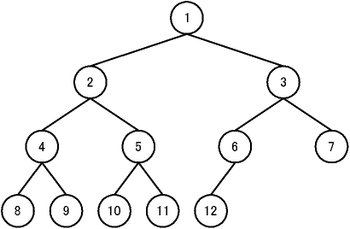
\includegraphics[scale=0.4]{Binary_heap_indexing}
 \begin{block}{Definition}
  Ein Binärbaum H ist ein Min-Heap, wenn für jeden Knoten $i$ mit $i \neq \text{root}$ gilt:
  $$\text{key}(H,i) \geq \text{key}(H,\text{parent}(i)$$
  und jede Schicht, bis auf die letzte, ausgefüllt ist.
  Wobei \verb|parent(i)| den Elterknoten von $i$ zurückgibt.
 \end{block}

\end{frame}

\begin{frame}{Binary Heap -- Aufgabe}
Geben sie jeden möglichen Max Heap zu den Zahlen 1,4,3,9,6 an.
\end{frame}

\begin{frame}{Bulk Insertion bei binären Heaps}
Gegeben sei ein binärer Heap, der n Elemente enhält. Es sollen nun k Elemente auf einmal
eingefügt werden. Geben Sie ein Verfahren an (kein Pseudocode), mit dem man das Einfügen in $\Oh(\min\{k \log k + \log n, k + \log n \log k \})$ Schritten erledigen kann.
Sie können davon ausgehen, dass der Heap genau $2m - 1$ enthält ($m \in \N$).
\end{frame}

\begin{frame}{Bulk Insertion bei binären Heaps -- Lösung}
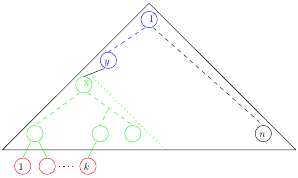
\includegraphics[scale=0.7]{bulkheap}
\begin{itemize}
 \item Falls $k \in \Omega(n)$:
 \begin{itemize}
  \item Rufe auf $k+n$ Elementen die Funktion buildHeap auf.
  \item Laufzeit $\Oh(k)$
 \end{itemize}
  \item k wesentlich kleiner als n:
  \begin{itemize}
   \item Verletze Heap-Eigenschaft: Hänge an den Heap an.
   \item Def x letzter Knoten der gemeinsamen Knoten aus k
   \item Für y = par(x): N ist von 1 bis y sortiert.
   \item $\bar{k}$ kleinste Zweierpotenz mit $k \leq \bar{k}$
   \item an T $\bar{k} - 1 < 2k \in \Oh(k)$
   \item es gibt $\lceil \log n \rceil - \lceil \log k \rceil + 1 \in \Oh(\log n)$ gemeinsame Vorgänger von K.
  \end{itemize}

\end{itemize}

  
 Sei K die Menge der einzufügenden Elemente. Man kann nun einfach die Elemente aus K hinten
 
\end{frame}

\begin{frame}{Bulk Insertion bei binären Heaps -- Lösung (2)}
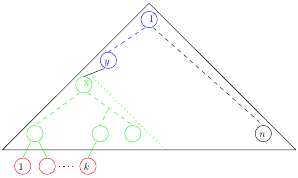
\includegraphics[scale=0.5]{bulkheap}
Für $k \leq \log n$
\begin{itemize}
 \item Muss in $\Oh(k \log k + \log n)$ liegen
 \item Finde x in $\Oh(\log n)$
 \item Schneide T aus Heap aus und sortiere $K \cup T$ in $\Oh(k \log k)$.
 \item Schneide N aus Heap aus. Merge N und $K \cup T$ in $\Oh(k + \log n)$.
 \item Füge nacheinander die kleinsten Elemente von $N \cup K \cup T$ in den 
 Heap ein. Beginne bei ursprünglichen Stelle von 1, fahre fort bis zur ursprünglichen Stelle von y.
 Füge die sortierten Elemente in den Teilheap ab der ursprünglichen Stelle von x ein.
 
 \item $\Oh(k + \log n)$
 
\end{itemize}
\end{frame}

\begin{frame}{$k > \log n$}
 
 \begin{itemize}
  \item $\Oh(k + \log n \log k)$
  \item Finde x in
  \item Schneide T aus, führe $K \cup T$ in $\Oh(k)$ Schritten buildHeap.
  \item Der Heap hat eine Größe $\Oh(k)$.
  \item Entnehme die N kleinsten Elemente aus dem Heap von $K \cup T$.
  \item Benötigt $\Oh(\log n \log k)$
  \item Schneide N aus dem Heap aus. Erhalte Sortierung in N.
  \item Merge N und M. $\Oh(\log n)$.
 \item Füge nacheinander die kleinsten Elemente von $N \cup K \cup M$ in den 
 großen Heap ein. Beginne bei ursprünglichen Stelle von 1, fahre fort bis zur ursprünglichen Stelle von y.
 \item Füge die sortierten Elemente in den Teilheap ab der ursprünglichen Stelle von x ein.
 \item Füge die restlichen Elemente per Standardfunktion ein.
 \item Verbinde $K \cup T$ und den gr. Heap. Konstante Zeit.
 \end{itemize}
$\Oh(k + \log n \log k)$
\end{frame}

\section{Pancake Sorting}
\begin{frame}[fragile]{Pancake-Sorting}
 Gegeben sind n Pancakes in unterschiedlicher Größe und gestapelt. Man hat einen Pancakeflipper zur Verfügung mit dem man
 die obersten l Pancakes umdrehen kann.
 Entwickelt einen schnellen Algorithmus, um die Pancakes umzudrehen.
\end{frame}

\begin{frame}[fragile]{Pancake-Sorting}
 \begin{itemize}
  \item Flippe den gr. Pancake ganz noch oben
  \item Flippe den ganzen Stapel usw.. 
 \end{itemize}
{ \Huge ?} 
\begin{verbatim}
https://www.youtube.com/watch?v=kk-_DDgoXfk
\end{verbatim}

\end{frame}

\begin{frame}{(a, b) - Bäume}
Visualisierung
 
\end{frame}



\end{document}
